\section{Rviz}
Continuaremos con lo anteriore. Veremos cómo podemos abrir el programa de visualización rviz utilizando el launch file.

Creamos una carpeta \texttt{rviz} al lado de la carpeta \texttt{urdf}. Luego abrimos rviz en terminal con el comando \texttt{rviz2}.

\begin{center}
    \begin{Verbatim}[gobble=4]
    rviz2
    \end{Verbatim}
\end{center}

Dentro de rviz, en el menú superior, en file, seleccionar Save Config As, como se muestra en la siguiente imagen:

\begin{figure}[H] 
    \centering    
    \makebox[\textwidth][c]{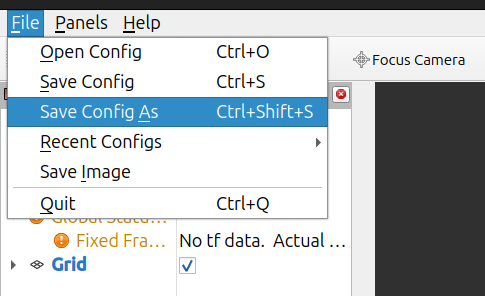
\includegraphics[width=1.4\textwidth]{imagenes/file-save-config.png}}
    \caption{rviz2, file, save config as.}
    \label{fig:mi_imagen}
\end{figure}

luego nombrar al archivo como panel.rviz, y guardar ese archivo en la carpeta \texttt{rviz} que acabamos de crear, como se muestra en la siguiente imagen:

\begin{figure}[H] 
    \centering    
    \makebox[\textwidth][c]{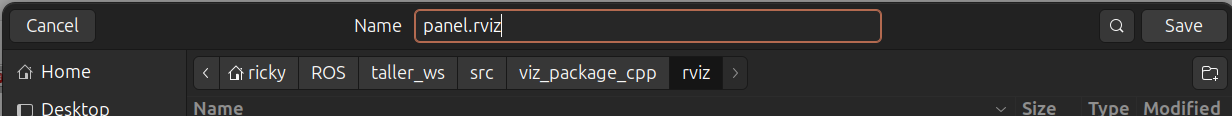
\includegraphics[width=1.4\textwidth]{imagenes/save-config2.png}}
    \caption{Guardamos archivo panel.rviz en la carpeta rviz.}
    \label{fig:mi_imagen}
\end{figure}

Ahora vamos a agregar esta nueva carpeta \texttt{rviz} al install del archivo CMakeLists.txt, como se muestra en la siguiente imagen.

\begin{figure}[H]
    \centering
    \makebox[\textwidth][c]{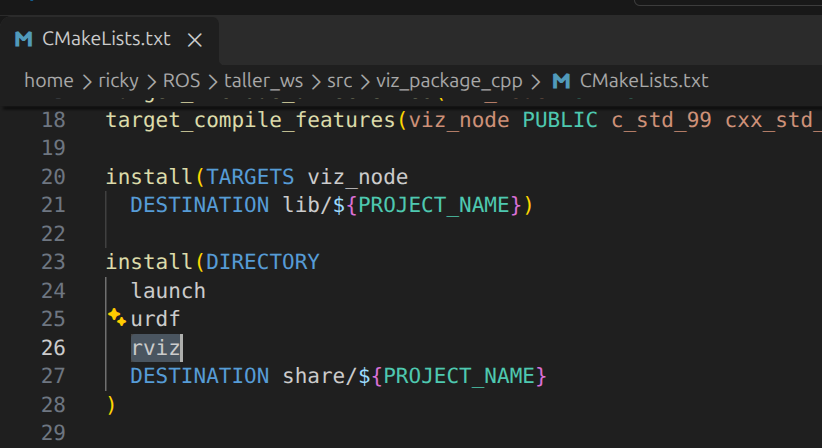
\includegraphics[width=1.4\textwidth]{imagenes/install-rviz-cmake.png}}
    \caption{Agregamos rviz al install del CMakeLists.txt}
    \label{fig:mi_imagen}
\end{figure}

Luego, agregamos un nuevo nodo en el launch file del paquete, este nodo abrirá rviz2 cuando se ejecute. Modificamos el launch file como se ve en la siguiente imagen:

\begin{figure}[H]
    \centering
    \makebox[\textwidth][c]{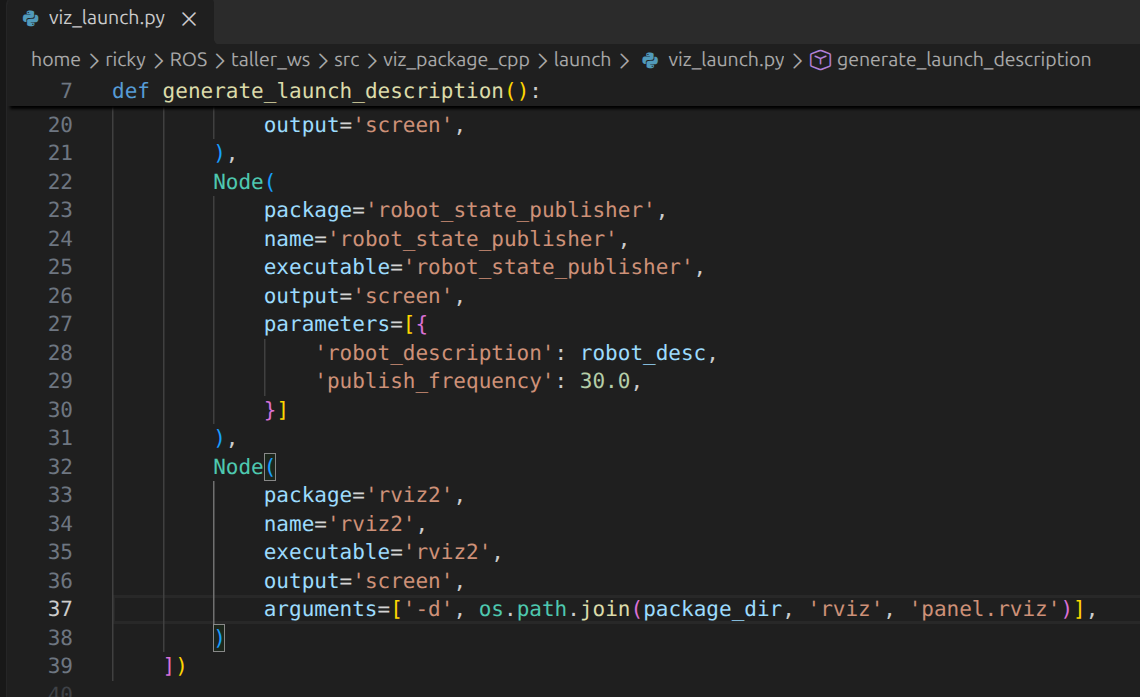
\includegraphics[width=1.4\textwidth]{imagenes/launch-rviz.png}}
    \caption{}
    \label{fig:mi_imagen}
\end{figure}

Ahora, en la terminal 1 compilamos con \texttt{colcon build}, en la terminal 2 lanzamos el launch file con \texttt{ros2 launch viz\_package\_cpp viz\_launch.py}. Esto se muestra en las siguientes imagenes:

\begin{figure}[H]
    \centering
    \makebox[\textwidth][c]{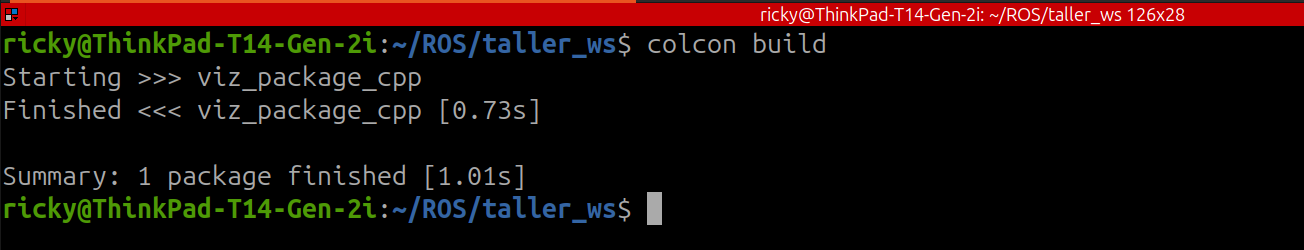
\includegraphics[width=1.4\textwidth]{imagenes/1:3-1.png}}
    \caption{}
    \label{fig:mi_imagen}
\end{figure}

\begin{figure}[H]
    \centering
    \makebox[\textwidth][c]{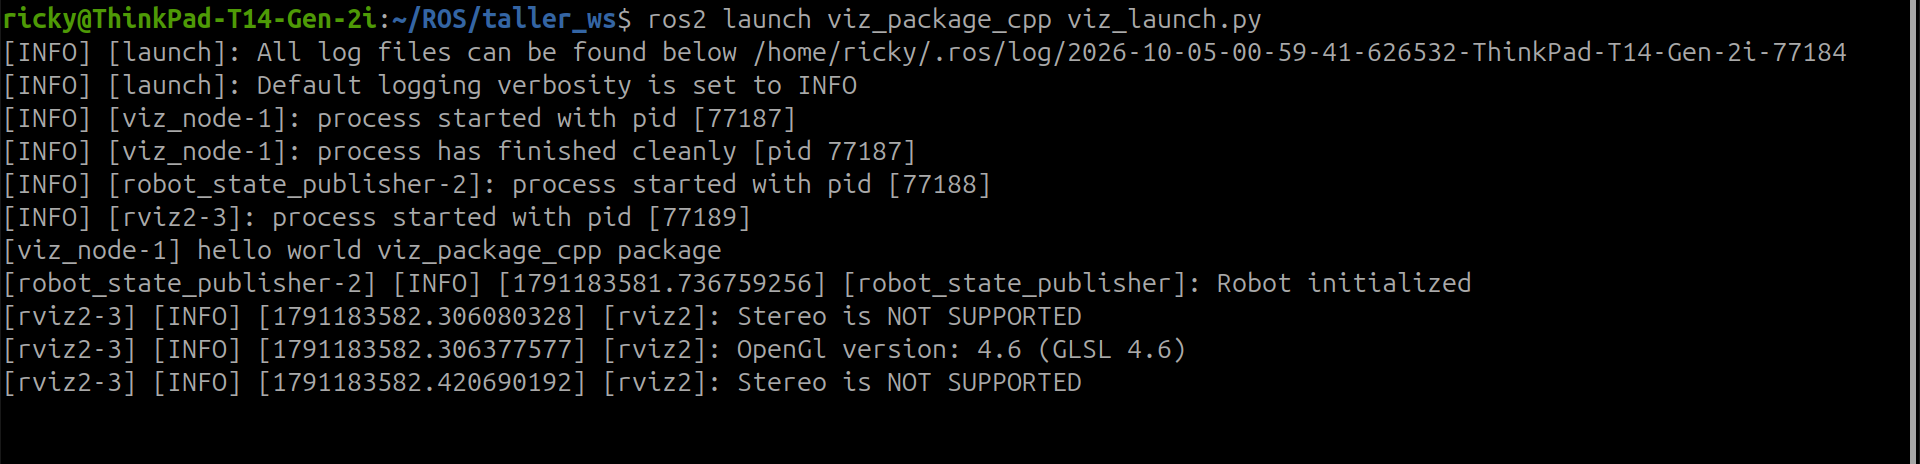
\includegraphics[width=1.4\textwidth]{imagenes/1:3-2.png}}
    \caption{}
    \label{fig:mi_imagen}
\end{figure}

\begin{figure}[H]
    \centering
    \makebox[\textwidth][c]{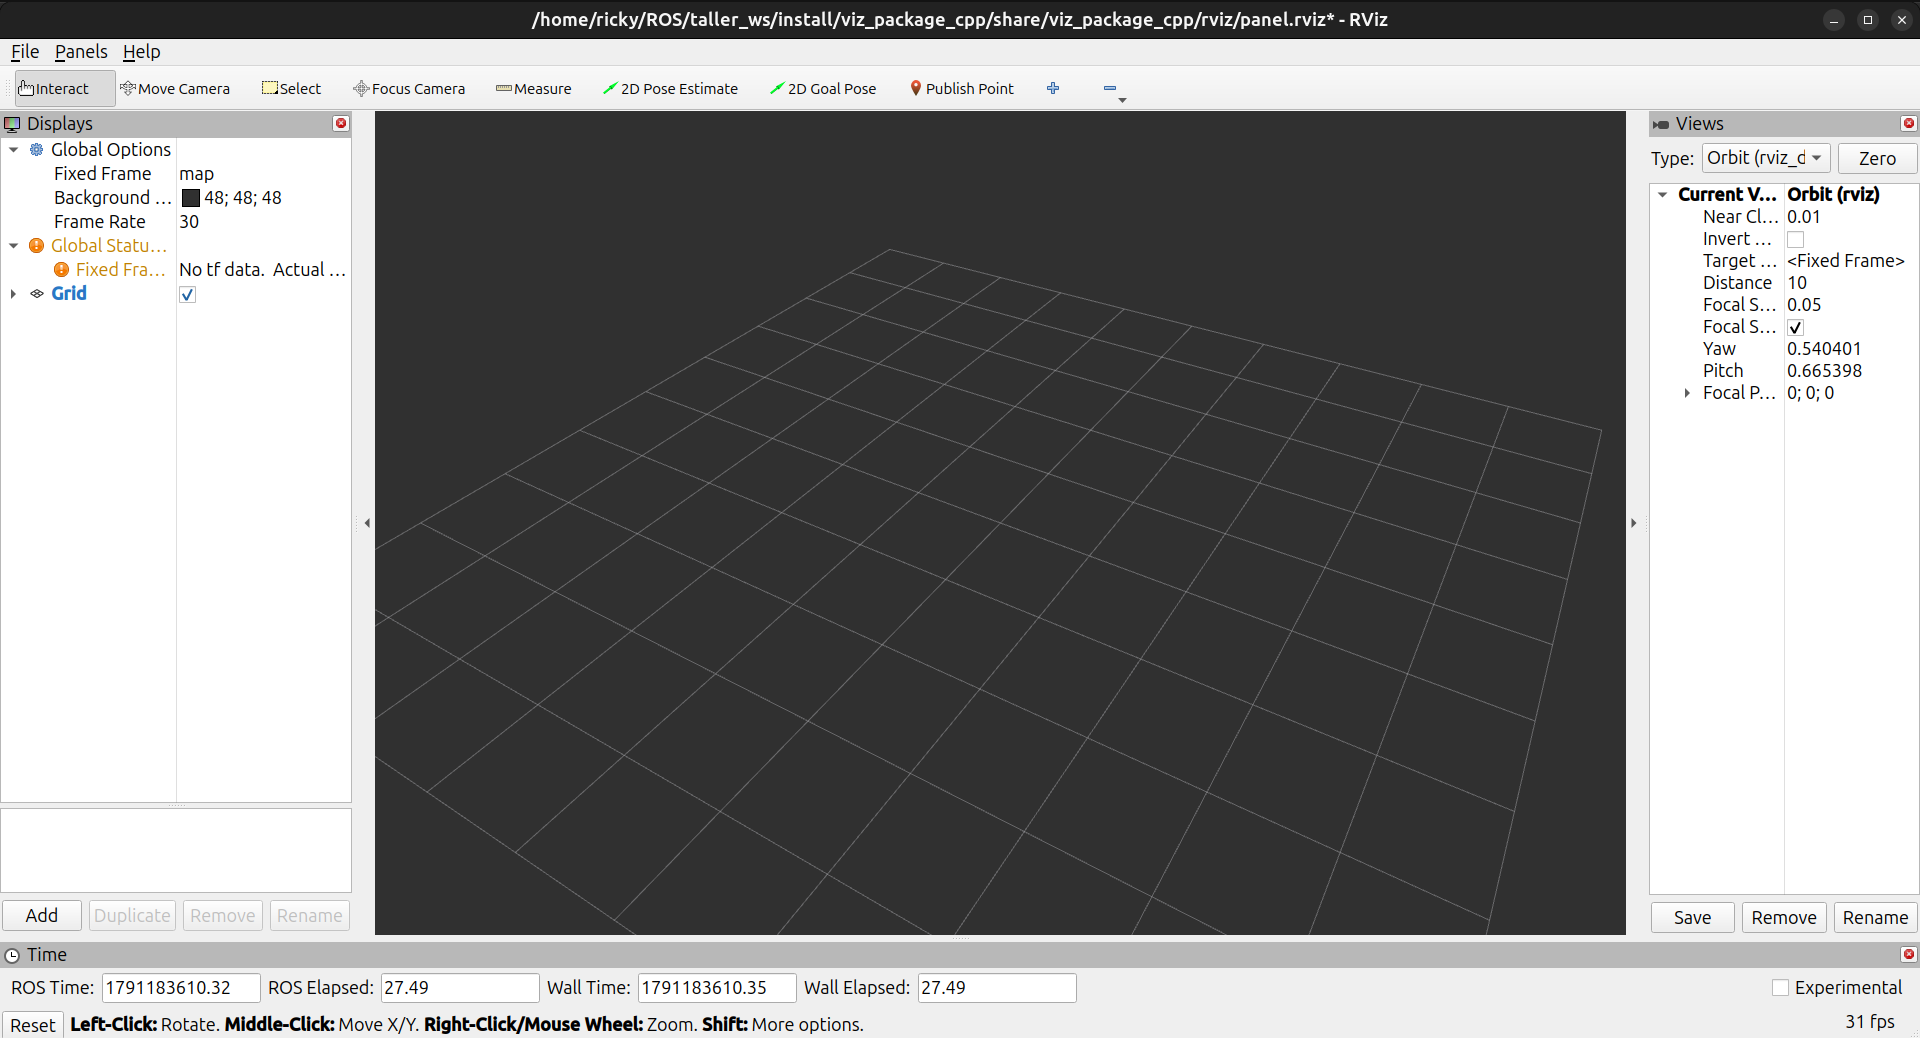
\includegraphics[width=1.4\textwidth]{imagenes/1:3-3.png}}
    \caption{}
    \label{fig:mi_imagen}
\end{figure}

Ahora, con el rviz abierto, en el menú de la izquierda, en la parte que dice Displays, seleccionamos el campo a la derecha de donde dice Fixed Frame, y cambiamos lo que dice map a base\_link. Esto se muestra en las siguientes imágenes:

\begin{figure}[H]
    \centering
    \makebox[\textwidth][c]{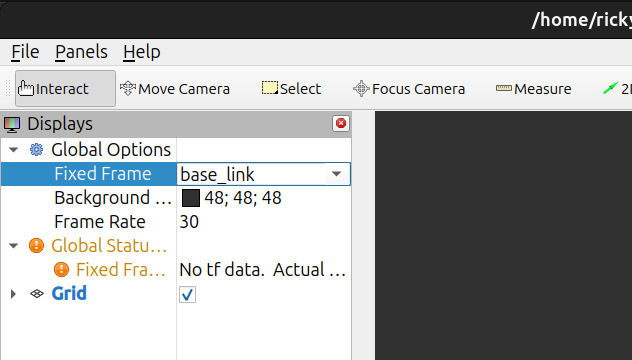
\includegraphics[width=1.4\textwidth]{imagenes/ffbl.png}}
    \caption{}
    \label{fig:mi_imagen}
\end{figure}

Ahora, en rviz, seleccionamos el boton que dice Add (que está abajo a la izquierda), y en la pestaña que dice By Display Type, seleccionamos RobotModel. Como se ve en la siguiente imagen:

\begin{figure}[H]
    \centering
    \makebox[\textwidth][c]{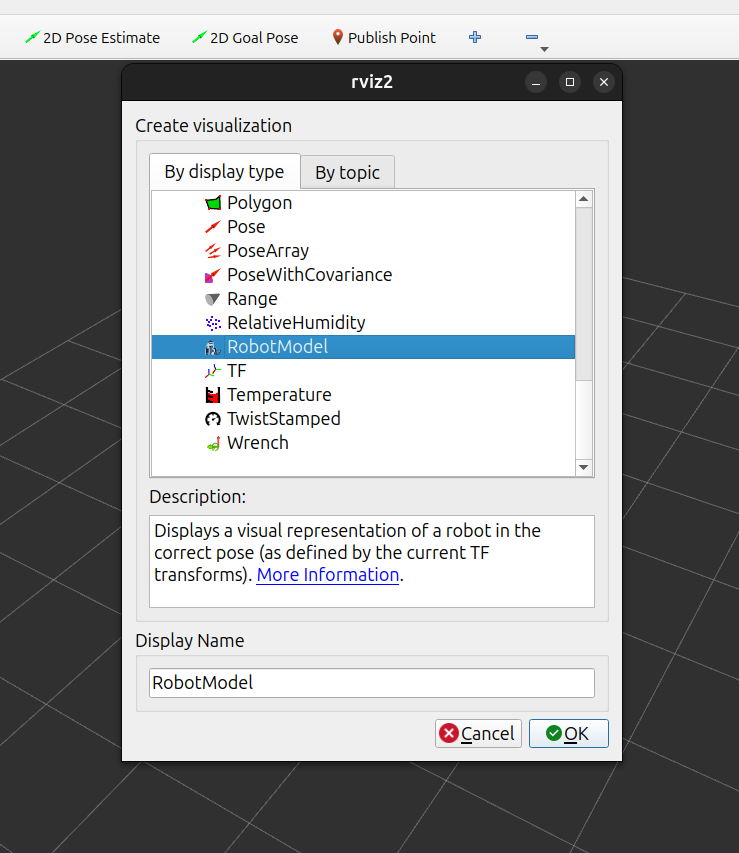
\includegraphics[width=1.4\textwidth]{imagenes/rmodel.png}}
    \caption{}
    \label{fig:mi_imagen}
\end{figure}

Ahora, en el menu de la izquierda aparecerá en un nuevo apartado que dice RobotModel, y en la opción Description topic, seleccionamos la opción que dice /robot\_description. Como se muestra en la imagen siguiente:

\begin{figure}[H]
    \centering
    \makebox[\textwidth][c]{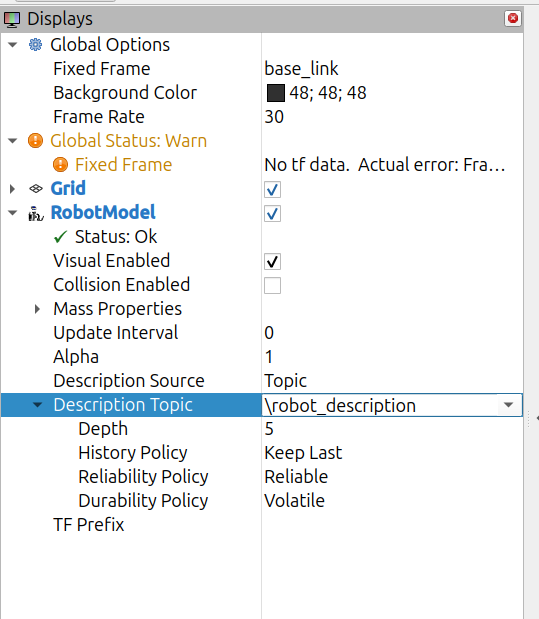
\includegraphics[width=1.4\textwidth]{imagenes/rdescriptionrviz.png}}
    \caption{}
    \label{fig:mi_imagen}
\end{figure}


Con las configuraciones anteriores, se debería de mostrar la pieza (nuestro robot hasta ahora) que definimos anteriormente en el archivo .urdf. 

\begin{figure}[H]
    \centering
    \makebox[\textwidth][c]{\includegraphics[width=1.4\textwidth]{imagenes/pieza.png}}
    \caption{}
    \label{fig:mi_imagen}
\end{figure}

